% \documentclass{book}

\documentclass[12pt]{article}
\usepackage[pdfborder={0 0 0.5 [3 2]}]{hyperref}%
\usepackage[left=1in,right=1in,top=1in,bottom=1in]{geometry}%
\usepackage[shortalphabetic]{amsrefs}%
\usepackage{amsmath}
\usepackage{enumerate}
\usepackage{enumitem}
\usepackage{amssymb}                
\usepackage{amsmath}                
\usepackage{amsfonts}
\usepackage{amsthm}
\usepackage{bbm}
\usepackage[table,xcdraw]{xcolor}
\usepackage{tikz}
\usepackage{float}
\usepackage{booktabs}
\usepackage{svg}
\usepackage{mathtools}
\usepackage{cool}
\usepackage{url}
\usepackage{graphicx,epsfig}
\usepackage{makecell}
\usepackage{array}

\def\noi{\noindent}
\def\T{{\mathbb T}}
\def\R{{\mathbb R}}
\def\N{{\mathbb N}}
\def\C{{\mathbb C}}
\def\Z{{\mathbb Z}}
\def\P{{\mathbb P}}
\def\E{{\mathbb E}}
\def\Q{\mathbb{Q}}
\def\ind{{\mathbb I}}

\graphicspath{ {images2/} }

\begin{document}
\section*{09 Jan 2017}

Apparently for my eigenvalues/eigenvectors from before, I accidentally used the double soliton before running it through the Newton solver instead of after. Good news: even though we get slightly different eigenvalues for pulses joined at the first min/max, the results are qualitatively the same. \\

Here are the results for the double pulse constructed by joining at the first min/max; this time we ran it through the Newton solver!

\begin{enumerate}
	\item Pulses joined at first min/max, 2nd order finite difference with Neumann BCs on $[0, 50]$ and extended by symmetry to $[-50, 50]$, eigenvalues/eigenvectors found using \textrm{eig}. Eigenvalues on the real axis are $0.011997, -0.011997$. Let $\lambda$ and $-\lambda$ be the two eigenvalues. Let $v(x)$ be the eigenfunction corresponding to $\lambda$. Then from the Matlab plots and data, the eigenfunction corresponding to $-\lambda$ is $v(-x)$, as expected. Note that in the Matlab plot, the eigenfunction corresponding to $-\lambda$ is actually $-v(-x)$, but this is okay since eigenfunctions only specified up to a scalar multiple. We get the same eigenvalues and eigenfunctions if we use \textrm{nobalance} or \textrm{eig}.

	\begin{figure}[H]
	\includegraphics[width=8.5cm]{double1_FD50.eps}
	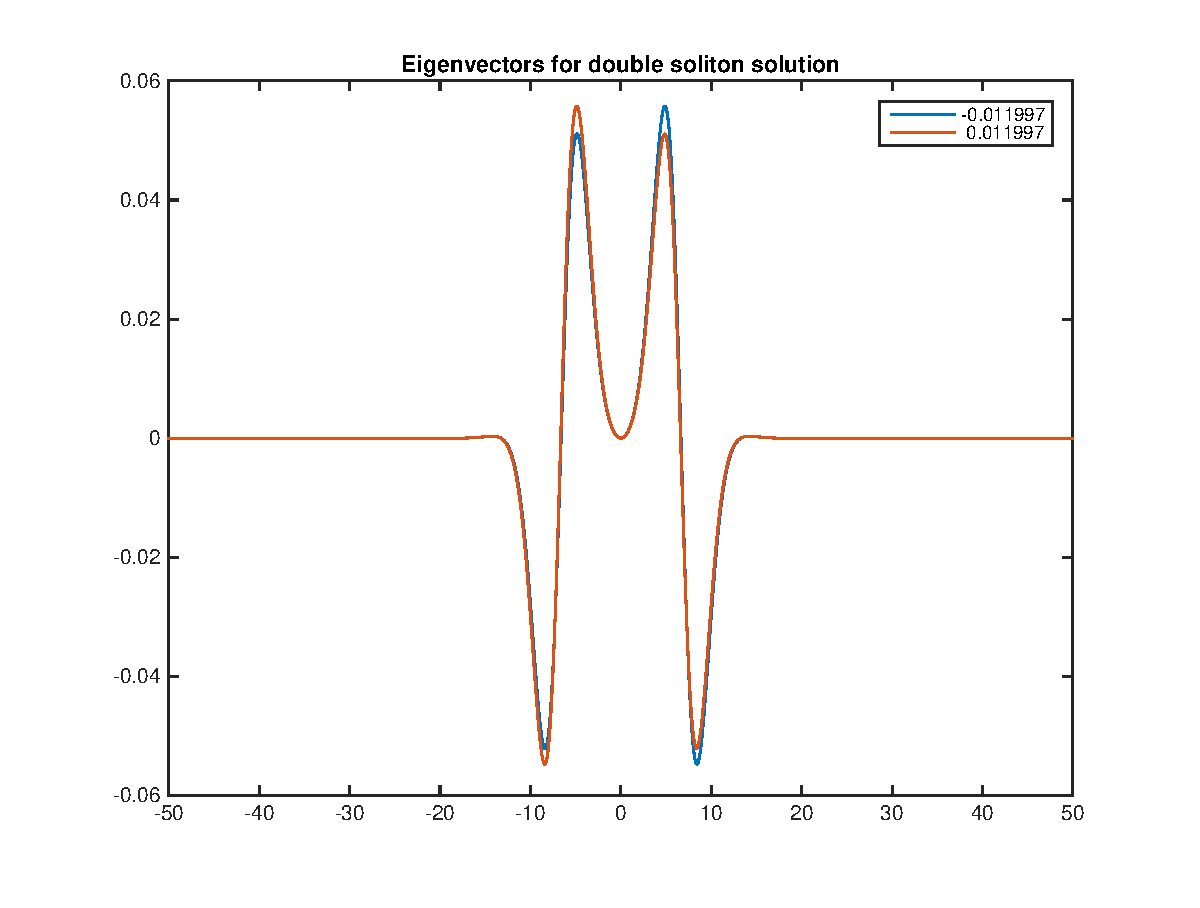
\includegraphics[width=8.5cm]{double1_FD50_vec.eps}
	\end{figure}

	\begin{figure}[H]
	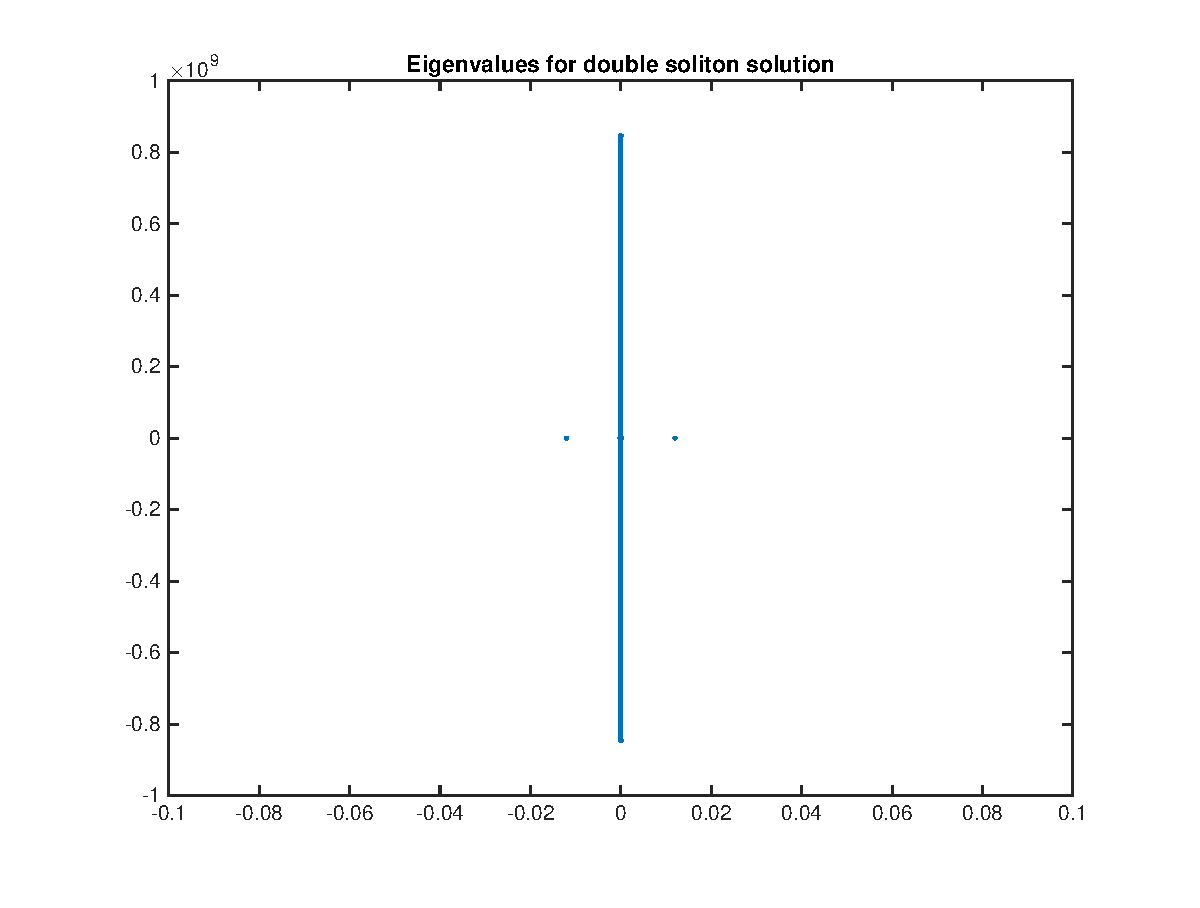
\includegraphics[width=8.5cm]{double1_FD50_eig.eps}
	\includegraphics[width=8.5cm]{double1_FD50_zoom.eps}
	\end{figure}

	We note in addition that there we find two small eigenvalues of order 1e-4 which are on the real axis. These are not exact negatives of each other, and I think it's likely that they are numerical artifacts.

	\item Extend domain of half-wave to $[0,100]$ (2000 grid points) and full wave to $[-100, 100]$. In other words, more ``zero-padding'' around our solitary wave. Everything else was the same. We have to use \textrm{eigs} instead of \textrm{eig} since the latter is too slow with this many grid points. The continuation method gives us a single puse for $c = 1.5647$, very close to the $c = 1.5650$ used above. We then construct double pulses as we did above. Since we used \textrm{eigs}, we will plot the eigenvalues here. As above, we have a pair of real eigenvalues at $0.012042, -0.012042$. In this case, no other very small real eigenvalues, only these two. They are very close to the above, the difference explainable by slightly different $c$. 

	\begin{figure}[H]
	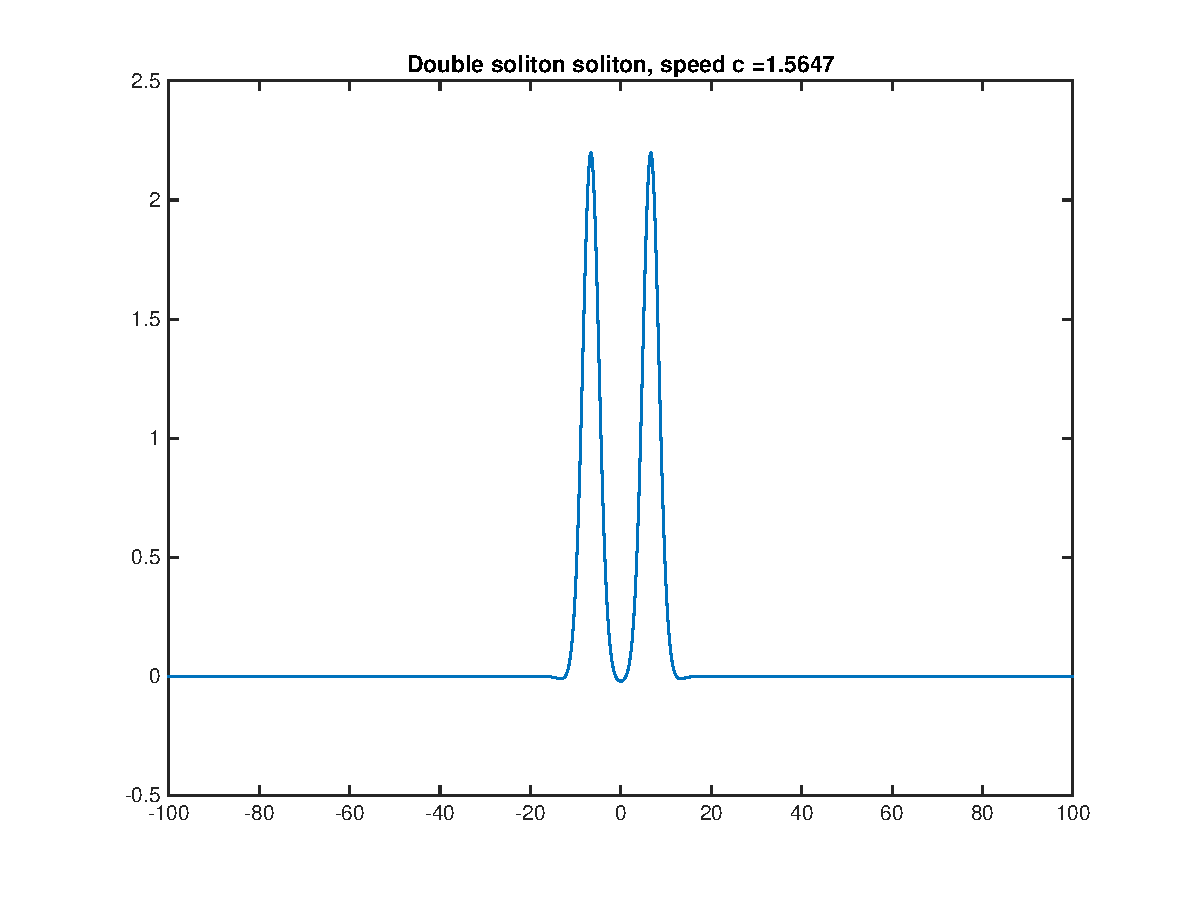
\includegraphics[width=8.5cm]{double1_FD100.eps}
	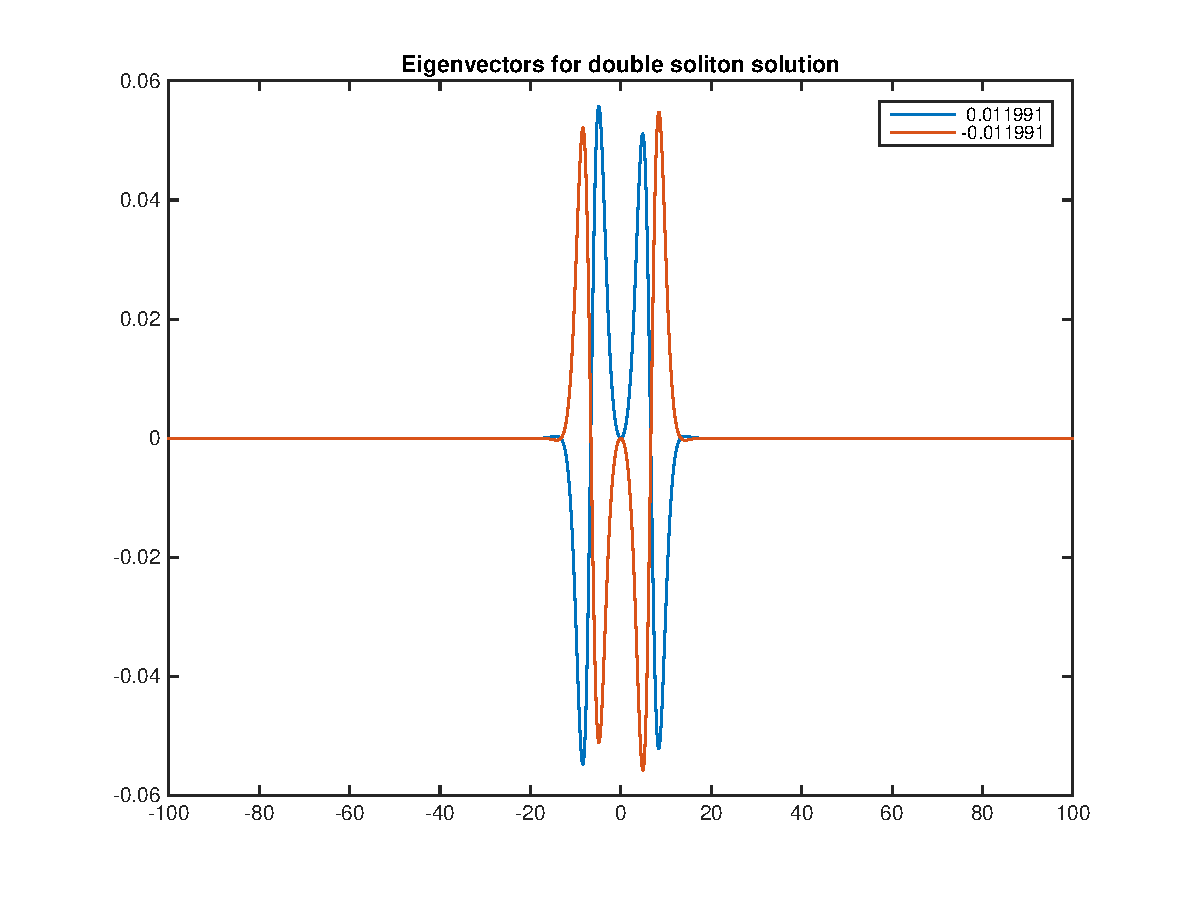
\includegraphics[width=8.5cm]{double1_FD100_vec.eps}
	\end{figure}

	Eigenvalues are almost identical to the case above on $[-50,50]$. Eigenfunctions are almost identical as well; the plot looks different, but if we take the second eigenfunction and multiply it by -1, the plot looks the same.

	\begin{figure}[H]
	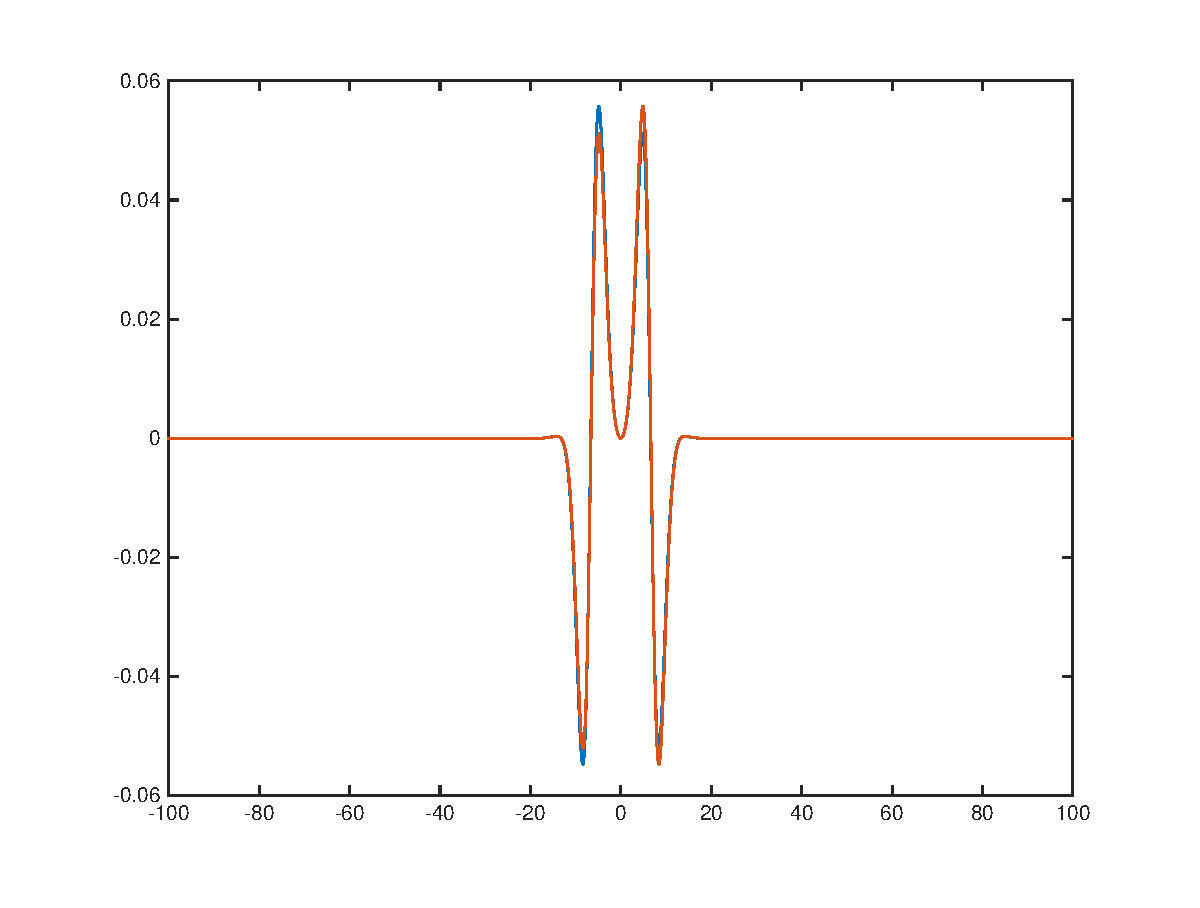
\includegraphics[width=8.5cm]{double1_FD100_vec2.eps}
	\end{figure}

	\item Repeat this using Fourier spectral methods (periodic BCs). Domain is always $[0, 2 \pi]$, but we rescaled to map $[-50, 50]$ to $[0, 2 \pi$. Continuation code run on 128 grid points, ramped up to 1024 grid points for creation of double soliton and eigenvalue experiments. Was able to get $c = 1.5672$ by continuation code, whics is very to close to what we had in the two cases above. 

	\begin{figure}[H]
	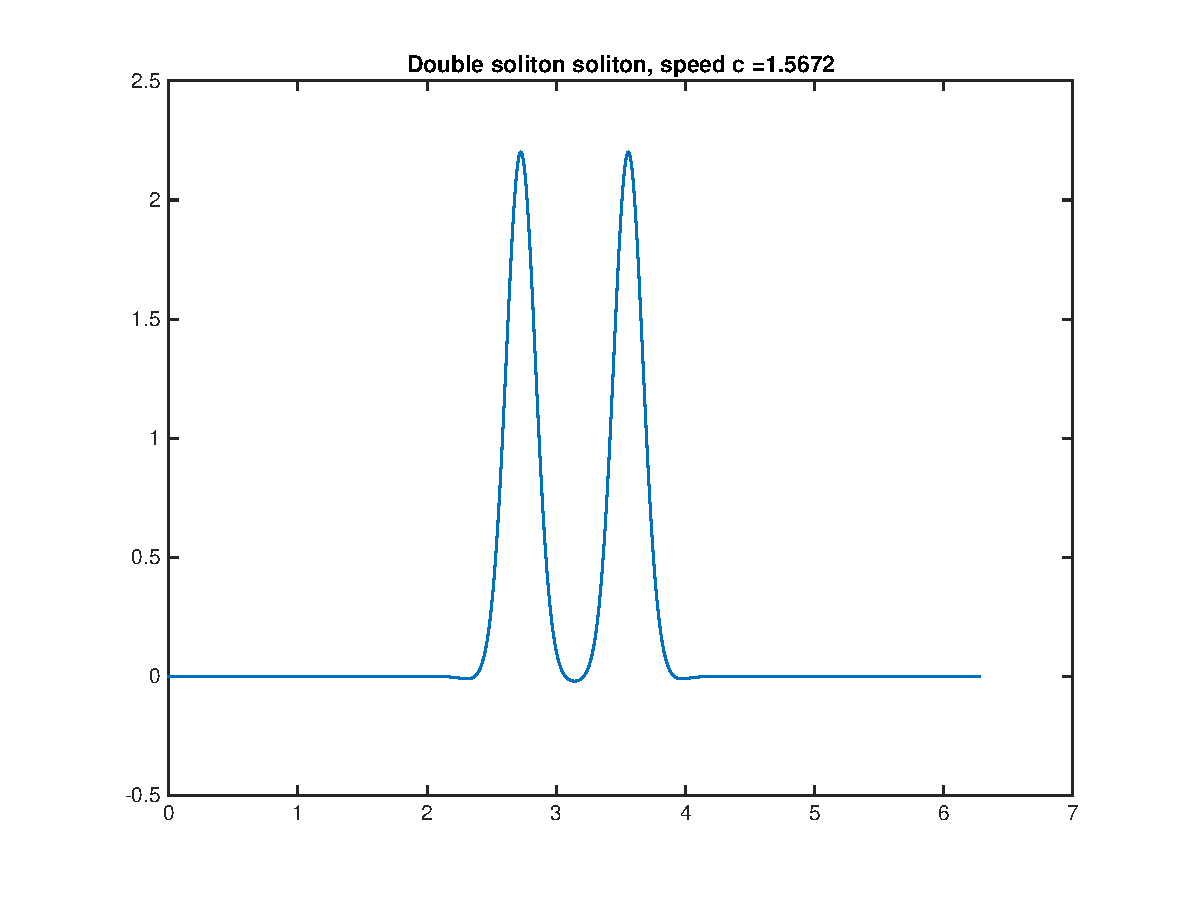
\includegraphics[width=8.5cm]{double1_Four50.eps}
	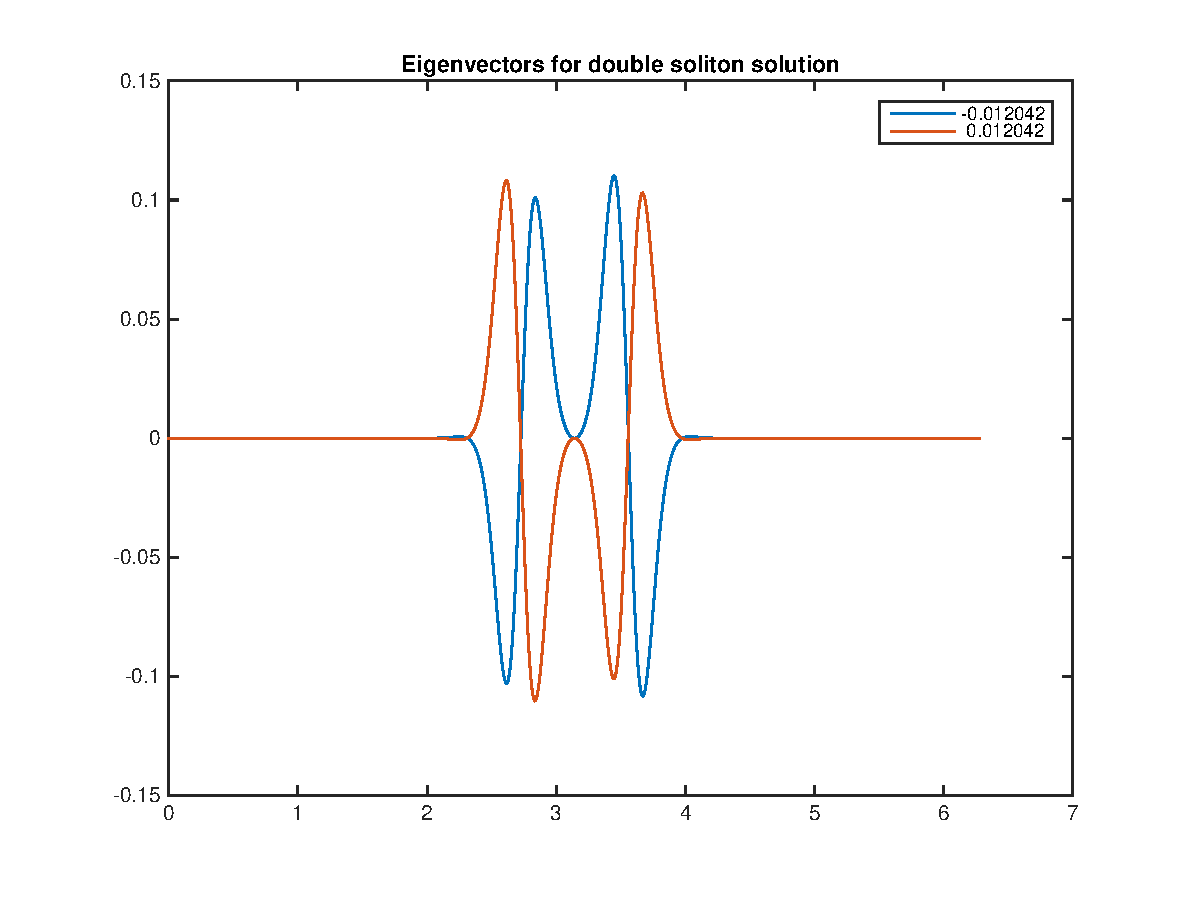
\includegraphics[width=8.5cm]{double1_Four50_vec.eps}
	\end{figure}

	\begin{figure}[H]
	\includegraphics[width=8.5cm]{double1_Four50_eig.eps}
	\includegraphics[width=8.5cm]{double1_Four50_zoom.eps}
	\end{figure}

\end{enumerate}

For all methods, for double pulse constructed this way (join at first min/max, so closest possible join), we get essentially the same eigenvalues and eigenfunctions. Eigenfunctions (interestingly) are not symmetric, but from inspection it looks like they will integrate to 0 as expected. A quick check using trapezoid rule shows this is the case.

\end{document}

